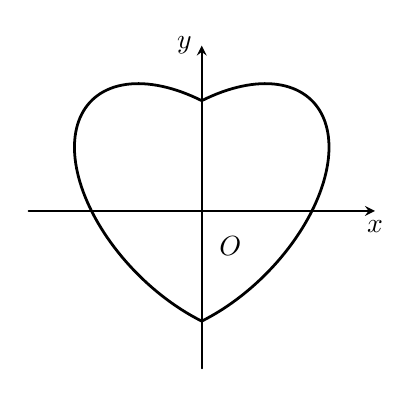
\begin{tikzpicture}[baseline,line cap=round,line join=round,>=stealth]
  \def\s{1.4}

  % Axes
  \draw[->,line width=0.6pt] (-2.2,0) -- (2.2,0) node[below] {$x$};
  \draw[->,line width=0.6pt] (0,-2.0) -- (0,2.1) node[left] {$y$};

  % Label Origin
  \node[below right] at (0.1,-0.2) {$O$};

  % Curve: x^2 + y^2 = 1 + |x|y
  % Right half (x >= 0): x = (2/sqrt(3))*cos(t), y = (1/sqrt(3))*cos(t) + sin(t), t in [-90, 90]
  % Left half (x <= 0): x = -(2/sqrt(3))*cos(t), y = (1/sqrt(3))*cos(t) + sin(t), t in [90, -90]
  \draw[line width=1.0pt]
    plot[domain=-90:90, samples=80] ({\s*(2/sqrt(3))*cos(\x)}, {\s*((1/sqrt(3))*cos(\x) + sin(\x))})
    --
    plot[domain=90:-90, samples=80] ({-\s*(2/sqrt(3))*cos(\x)}, {\s*((1/sqrt(3))*cos(\x) + sin(\x))})
    -- cycle;
\end{tikzpicture}
